\documentclass[12pt]{beamer}
\usepackage{graphicx}
\usepackage{fancyvrb}
\fvset{fontsize=\normalsize}
\usepackage{multicol}
\usepackage{booktabs}
\usepackage{units}
\usepackage[T1]{fontenc}
\usepackage[utf8]{inputenc}
\usepackage{helvet}
\usepackage{multicol}
\usepackage{amsmath}
\usepackage{mathtools}
\usepackage{changepage}

\usetheme{default}
\beamertemplatenavigationsymbolsempty
\hypersetup{pdfpagemode=UseNone} 
\setbeameroption{hide notes}
\setbeamertemplate{note page}[plain]

\usetheme{default}
\beamertemplatenavigationsymbolsempty
\hypersetup{pdfpagemode=UseNone} % don't show bookmarks on initial view


\usefonttheme{professionalfonts}
\usefonttheme{serif}
\fontfamily{sans}
\setbeamerfont{note page}{family*=pplx,size=\footnotesize} % Palatin

\definecolor{foreground}{RGB}{245,245,245}
\definecolor{white}{RGB}{255,255,255}
\definecolor{background}{RGB}{24,24,24}
\definecolor{title}{RGB}{107,174,214}
\definecolor{gray}{RGB}{135,135,135}
\definecolor{subtitle}{RGB}{102,255,204}
\definecolor{hilight}{RGB}{102,255,204}
\definecolor{vhilight}{RGB}{255,111,207}
\definecolor{carrotorange}{rgb}{240,145,50}
\definecolor{yuppiered}{RGB}{230,79,43}
\setbeamercovered{transparent}

\setbeamercolor{titlelike}{fg=title}
\setbeamercolor{subtitle}{fg=subtitle}
\setbeamercolor{institute}{fg=gray}
\setbeamercolor{normal text}{fg=foreground,bg=background}

\setbeamercolor{item}{fg=foreground} % color of bullets
\setbeamercolor{subitem}{fg=gray}
\setbeamercolor{itemize/enumerate subbody}{fg=gray}
\setbeamertemplate{itemize subitem}{{\textendash}}
\setbeamerfont{itemize/enumerate subbody}{size=\footnotesize}
\setbeamerfont{itemize/enumerate subitem}{size=\footnotesize}
\setbeamertemplate{footline}{%
    \raisebox{5pt}{\makebox[\paperwidth]{\hfill\makebox[20pt]{\color{gray}
          \scriptsize\insertframenumber}}}\hspace*{5pt}}

\addtobeamertemplate{note page}{\setlength{\parskip}{12pt}}

\title{Nonparametric covariance estimation for longitudinal data via tensor product smoothing}
\author{Tayler Blake \inst{1} \and Dr. Yoonkyung Lee \inst{2}}
\institute{\inst{1} Information Control Company \and %
                      \inst{2} The Ohio State University, Department of Statistics}

\setbeamertemplate{footline}{%
    \raisebox{5pt}{\makebox[\paperwidth]{\hfill\makebox[20pt]{\color{gray}
          \scriptsize\insertframenumber}}}\hspace*{5pt}}

% These commands are used to pretty-print LaTeX commands
\newcommand{\bi}{\begin{itemize}}
\newcommand{\ei}{\end{itemize}}
\newcommand{\ig}{\includegraphics}
\newcommand{\subt}[1]{{\footnotesize \color{subtitle} {#1}}}
\newcommand{\newthought}[1]{{\small \color{hilight} {#1}}}
\newcommand{\newmaththought}[1]{{ \color{foreground} {#1}}}
\newcommand{\carrotorangemath}[1]{{ \color{carrotorange} {#1}}}
\newcommand{\mixedmodelmath}[1]{{ \color{yuppiered} {#1}}}
\newcommand{\makegrey}[1]{{ \color{gray} {#1}}}
\newcommand{\makewhite}[1]{{ \color{white} {#1}}}
\newcommand{\ms}{\scriptscriptstyle}
\newcommand\cooloverbrace[2]{\mathrlap{\smash{%
\overbrace{\phantom{\begin{matrix} #2 %
\end{matrix}}}^{\mbox{$#1$}}}}#2}
\newcommand\coolunderbrace[2]{\mathrlap{\smash{%
\underbrace{\phantom{\begin{matrix} #2 %
\end{matrix}}}_{\mbox{$#1$}}}}#2}


\newcommand{\doccmd}[1]{\texttt{\textbackslash#1}}% command name -- adds backslash automatically
\newcommand{\docopt}[1]{\ensuremath{\langle}\textrm{\textit{#1}}\ensuremath{\rangle}}% optional command argument
\newcommand{\docarg}[1]{\textrm{\textit{#1}}}% (required) command argument
\newenvironment{docspec}{\begin{quote}\noindent}{\end{quote}}% command specification environment
\newcommand{\docenv}[1]{\textsf{#1}}% environment name
\newcommand{\docpkg}[1]{\texttt{#1}}% package name
\newcommand{\doccls}[1]{\texttt{#1}}% document class name
\newcommand{\docclsopt}[1]{\texttt{#1}}% document class option name

\newcommand\myfootnote[1]{%
  \begingroup
  \renewcommand\thefootnote{}\footnote{#1}%
  \addtocounter{footnote}{-1}%
  \endgroup
}





















\begin{document}

%1
{
\setbeamertemplate{footline}{} % no page number here
\frame{
  \titlepage
%  \note{These are slides for a talk I will give on 24 Oct 2013, at a
 %   symposium on open access publishing, organized by the Ebling
   % Library, UW{\textendash}Madison.}
}
}

%2
\begin{frame}
\frametitle{\emph{}}
\newthought{The data:}
\begin{equation*}
Y_i = \left( Y_{i1}, Y_{i2}, \dots, Y_{iM_i} \right)^\prime, \qquad i=1,\dots, N
\end{equation*}
\noindent
associated with measurement times 
\[
t_{1} < t_{2} < \dots< t_{M_i}.
\]

\newthought{Goal:} estimate
\[
Cov\left(Y\right) = \Sigma
\]

\end{frame}



%3
%3
%3
\begin{frame}
\frametitle{\emph{The flaming hoops:}}
\bi
\item Covariance matrices (and their estimates) should be positive definite.
	\begin{itemize}
	\item Constrained optimization is a headache.
	\end{itemize} \pause
\item The $\left\{t_{ij} \right\}$ may be suboptimal. 
\begin{itemize}
	\item Observation times may not fall on a regular grid, may vary across subjects.
	\end{itemize} \pause
\item More dimensions, more problems (maybe.)
\begin{itemize}
	\item Sample covariance matrix falls apart when $m$ is large.
	\end{itemize} 
\ei
\end{frame}




%4
%4
%4

%\begin{frame}
%\frametitle{\emph{The flaming hoops:}}
%\bi
%\item<4>Covariance matrices (and their estimates) should be positive definite.
%	\newthought{A cute little reparameterization } $\color{hilight} \Longrightarrow$ \newthought{unconstrained estimation, meaningful interpretation} 
%\item<5> The $\left\{t_{ij} \right\}$ may be messy. \\
%	\newthought{Frame covariance estimation as function estimation.} 
%\item<6>  More dimensions, more problems (maybe.) \\
%\begin{figure}
%\graphicspath{{img/}}
%  \includegraphics<6>[height=3cm]{ripnatedogg}
%  \only<6>{\caption{\color{hilight}\small Regulate like Nate Dogg.}}
%\end{figure}
%\ei
%\end{frame}

\begin{frame}
\frametitle{\emph{The flaming hoops:}}
\bi
\item Covariance matrices (and their estimates) should be positive definite.
	\newthought{A cute little reparameterization } $\color{hilight} \Longrightarrow$ \newthought{unconstrained estimation, meaningful interpretation} 
\item The $\left\{t_{ij} \right\}$ may be messy. \\
	\newthought{Frame covariance estimation as function estimation.} 
\item  More dimensions, more problems (maybe.) \\
\begin{figure}
\graphicspath{{img/}}
  
\includegraphics[height=3cm]{ripnatedogg}
  \only{\caption{\color{hilight}\small Regulate like Nate Dogg.}}
\end{figure}
\ei
\end{frame}


%5

\begin{frame}
\frametitle{\emph{Covariance dress-up: the modified Cholesky decomposition}}

\begin{equation*}
Y = \left(Y_1, \dots, Y_M \right)^\prime \sim \mathcal{N}\left(0,\Sigma\right).
\end{equation*}

\newthought{For any positive definite} $\color{hilight}{\Sigma}$, \newthought{we can find $T$ which diagonalizes} $\color{hilight}{\Sigma}$:

\begin{equation*}
D = T \Sigma T^\prime, \quad T = \begin{bmatrix} 1 & 0 & \dots & & \\ -\phi_{21} & 1 & & & \\ -\phi_{31}& -\phi_{32} &  1 & & \\ \vdots & & & \ddots & \\ -\phi_{M1} &-\phi_{M2} & \dots & -\phi_{M,M-1}& 1  \end{bmatrix}
\end{equation*}
%\myfootnote{The matrix $T$ is the \emph{Cholesy factor}  of the precision matrix.}
\end{frame}




\begin{frame}
\frametitle{}

\vfill
  \begin{beamercolorbox}[center]{title}
\Large Now, for the cutest part:
  \end{beamercolorbox}
  \vfill

\end{frame}




\begin{frame}
\frametitle{}
\begin{figure}
\graphicspath{{img/}}
  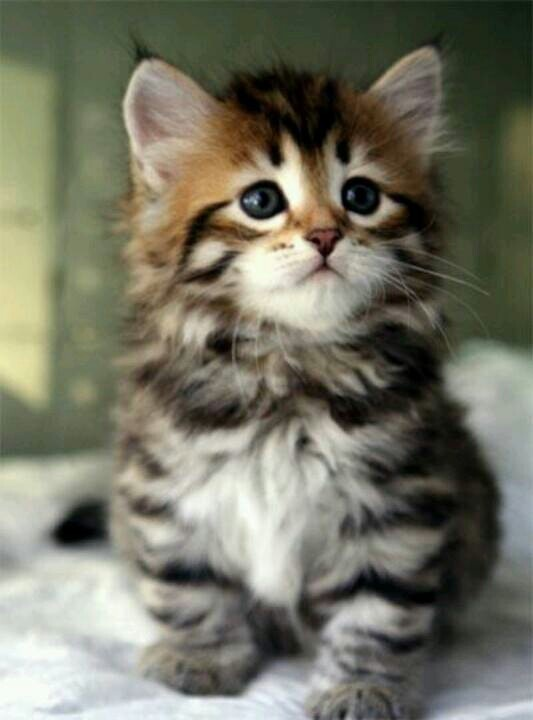
\includegraphics[height=9cm]{cutest-kitten-ever}
\end{figure}

\end{frame}

%6
\begin{frame}
\frametitle{\emph{Okay, really:}}

Regress $Y_j$ on $Y_{\ms{\left(1:j-1\right)}} = \left(Y_1, \dots, Y_{\ms{j-1}}\right)^\prime$:

\begin{align} \label{eq:ARmodel}
y_{j}  = \left\{  \begin{array}{ll} 
		e_1 &j=1, \\
  \sum \limits_{k=1}^{j-1} \phi_{jk} y_{k} + \sigma_{j}e_{j} &  j=2,\dots,M
\end{array}\right.
\end{align}
\noindent
In matrix form:
\begin{align}
%\begin{split}
\newmaththought{ e = TY,}
%\end{split}
\end{align}
\noindent
 and taking covariances on both sides:
\begin{equation}
\newmaththought{ D = \sigma_{\ms e}^2 \mbox{diag}\left( \sigma_1^2,\dots, \sigma_M^2 \right) = T \Sigma T^\prime.}
\end{equation}
\end{frame}








\begin{frame}
\frametitle{\emph{No constraints on the} $\phi_{jk}$s!}

\begin{adjustwidth}{-3cm}{-3cm}
\begin{center}
\begin{figure}
\graphicspath{{img/}}
  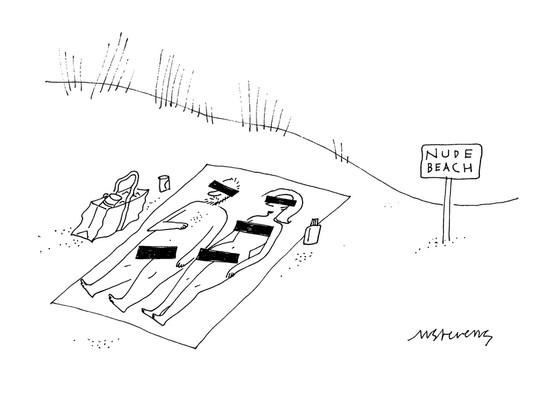
\includegraphics[height=7.5cm]{nude-beach}
\end{figure}
\end{center}
  \end{adjustwidth}
\end{frame}





\begin{frame}
\frametitle{\emph{The regression model tool box is a deep, luxurious toolbox.}}

\begin{align*}
\makegrey{Y_j}  	&\longrightarrow \makewhite{Y\left( t_j \right) }		&	 \makegrey{e_j} 		&\longrightarrow \makewhite{e\left( t_j \right)}\\
\makegrey{\phi_{jk}} &\longrightarrow \makewhite{\phi\left(t_j,t_k\right)} 	& 	\makegrey{\sigma^2_{j}} &\longrightarrow \makewhite{\sigma^2\left(t_j\right)}
\end{align*}
\noindent


\begin{equation}  \label{eq:MyModel}  
\makewhite{y\left(t_j \right)}  \makewhite{= \sum_{k=1}^{j-1} \phi\left(t_j ,t_k\right) y\left(t_k\right) + \sigma\left(t_j\right)e\left({t_j}\right)},
\end{equation}
\noindent
where
\begin{equation*} 
\makewhite{e\left(s\right)} \makewhite{ \sim  \mathcal{WN}\left(0,\sigma_{\ms e}^2 \right)}
\end{equation*}


%\myfootnote{The $\left\{ \phi_{jk} \right\}$ are called \emph{generalized autoregressive parameters}.}
%\myfootnote{The $\left\{ \sigma^2_{j} \right\}$ are called the \emph{innovation variances}.}
\end{frame}






\begin{frame}
\frametitle{\emph{Regularization of $\phi\left(s,t\right)$ is more intuitive if we transform the $s$-$t$ axis. }}

\begin{align*}
\newmaththought{l} &\newmaththought{= s-t} \\
\newmaththought{m} &\newmaththought{= \frac{1}{2}\left(s+t\right)}
\end{align*}
\noindent
Reparameterize $\phi$:
\begin{align*}
\newmaththought{\phi\left(s,t\right) =\phi^*\left(l,m\right)= \phi^*\left(s-t, \frac{1}{2}\left(s+t\right)\right)}
\end{align*}

Take $\hat{\phi}^*$ to be the minimizer of 
%\[
%\underbracket[0.2pt]{-2L}_{\text{\parbox{3cm}{\centering \mbox{ \;}\\ goodness \\[-4pt] of fit}}} + \underbracket[0.2pt]{\lambda J\left(\phi^*\right)}_{\text{\parbox{3cm}{\centering \mbox{ \;}\\ %flexibility of the \\[-4pt] fitted curve}}}
%\]
\begin{adjustwidth}{-2cm}{-2cm}
\begin{equation}
-2 L_\phi\left(\phi, y_1, \dots,y_N \right) = \sum_{i=1}^n \sum_{j=2}^{m_i} \sigma_{ij}^{-2} \left(y_{ij} - \sum_{k=1}^{j-1}\phi\left({t_{ij},t_{ik}}\right)y_{ik} \right)^2 \label{loglikelihood}
\end{equation}
\end{adjustwidth}

\end{frame}






%\begin{frame}
%\frametitle{\emph{Penalized maximum likelihood estimation}}
%
%\begin{enumerate}
%\item Fix $\sigma_{ij}^2 = \sigma_{ij0}^2$, $i=1,\dots,N$ ,$j=1,\dots,M$.
%\item Find $\phi_0 = \underset{\phi}{arg \; min} -2L_\phi\left(\phi, y_1,\dots, y_N \right) + \lambda J\left( \phi \right)$
%\item Fix $\phi = \phi_{0}$.
%\item Find  $\sigma_{0}^2 = \underset{\sigma^2}{arg\; min} -2L_\sigma^2\left(\sigma^2, y_1,\dots, y_N \right) + \lambda J\left( \sigma^2 \right)$
%\end{enumerate}
%
%\begin{adjustwidth}{-2cm}{-2cm}
%\begin{equation}
%-2 L_\phi\left(\phi, y_1, \dots,y_N \right) = \sum_{i=1}^N \sum_{j=2}^{m_i} \sigma_{ij0}^{-2} \left(y_{ij} - \sum_{k=1}^{j-1}\phi\left({t_{ij},t_{ik}}\right)y_{ik} \right)^2 \label{loglikelihood}
%\end{equation}
%\end{adjustwidth}
%\end{frame}





\begin{frame}
\frametitle{\emph{Smooth ANOVA models}}
Decompose
\begin{equation} \label{eq:SANOVA-model}
\carrotorangemath{
\phi^*\left(l,m\right) = \mu + \phi_1\left(l\right) + \phi_2\left(m\right) + \phi_{12}\left(l,m\right)},
\end{equation} 
so Model~\ref{eq:MyModel} becomes

\begin{align*}  
\begin{split}% \label{eq:expanded-ps-anova-vc-model}
 y\left(t_j \right)  = \sum_{k=1}^{j-1} \bigg[\mu + \phi_1\left(l_{jk}\right) +  &\phi_2\left(m_{jk}\right) \bigg.\\[-2ex]
\bigg. &+ \phi_{12}\left(l_{jk},m_{jk}\right) \bigg]y\left(t_k\right)+ \sigma\left(t_j\right)e\left({t_j}\right)
\end{split}
\end{align*}
\end{frame}


\begin{frame}
\frametitle{\emph{Approximate $\phi_1$, $\phi_2$, $\phi_{12}$ with B-splines.}}

\begin{align}  
\begin{split}\label{eq:l-m-marginal-basis}
\phi^*\left(l,m \right) &= B \theta \\
&= \phi_1\left(l\right)  + \phi_2\left(m\right)  + \phi_{12}\left(l,m\right)  \\
&= \sum_{c=1}^{c_l} B_{\ms c}\left(l\right) \theta_{lc }  B_{\ms l} \theta_l + \sum_{c^\prime=1}^{c_m} B_{\ms{c^\prime}}  \left(  m \right)  \theta_{\ms{mc^\prime }}  \\
&\mbox{\;\;\;\;\;\;\;\;\;\;\;\;\;\;\;\;\;\;\;\;\;\;\;\;\;\;\;\;\;\;} + \sum_{c=1}^{c_l} \sum_{{c^\prime}=1}^{c_m} B_{\ms c}\left(l\right) B_{\ms{c^\prime } }\left(m\right)\theta_{\ms{c c^\prime} } 
\end{split}
\end{align}

where $\theta \equiv \left(\mu, \theta_{\ms{l}},\theta_{\ms{m}},\theta_{\ms{lm}}\right)^\prime $ and
\begin{align*}
B &\equiv \left[\; 1_p \; \vert \;  B_l  \; \vert \;   B_m \; \vert B_{\ms{lm}} \; \right] \\
&= \left[\; 1_p \; \vert \;  B_l  \; \vert \;   B_m \; \vert  B_m \; \square \; B_l \right] 
\end{align*}

\end{frame}

%
%\begin{frame}
%\frametitle{\emph{PS-ANOVA model basis}}
%
%In matrix notation, Model \ref{eq:expanded-ps-anova-vc-model} becomes
%
%\begin{equation*}  
%E \left[ Y | W \right] = WB \theta,
%\end{equation*}
%\noindent
%where $W$ is the matrix of covariates holding the past values of $Y$, and $B$ is the $B$-spline regression basis:
%\begin{equation} \label{eq:SANOVA-basis-matrix}
%B = \left[\; 1_p \; \vert \;  B_l  \; \vert \;   B_m \; \vert B_{lm} \; \right]
%\end{equation}
%\noindent
%where 
%\begin{align*} \label{eq:rowwise-kronecker-product}
%B_{lm} &= B_m \; \square \; B_l \\
%&\equiv \left( B_m \otimes 1^\prime_{c_l} \right) \odot \left(1^\prime_{c_m} \otimes  B_l  \right).
%\end{align*}
%\end{frame}
%
%



%
%\begin{frame}
%\frametitle{\emph{Difference penalty had to regulate.}}
%
%For $f\left(x\right)=\sum \limits_{i=1}^{p} B_{i}\left(x\right) \theta_{i}$, approximate
%
%\begin{align}
%\begin{split}
%\int_0^1 \left(f^{\prime \prime}\left(x\right)\right)^{\ms 2} \;dx &= \int_0^1 \bigg\{ \sum \limits_{i=1}^{p} B^{\prime \prime}_{i}\left(x\right) \theta_{i} \bigg\}^{\ms 2} \;dx \\ 
%&= k_1 \newmaththought{\sum_i \left( \Delta^{\ms 2} \theta_i \right)^{\ms 2}} + k_2, 
%\end{split}
%\end{align}
%\noindent
%by
%\[
%\newmaththought{\vert \vert D_{\ms 2} \theta \vert \vert^{\ms 2}, \qquad  D_{\ms 2} \theta= \left( \Delta^{\ms 2}\theta_{\ms 1},\dots,\Delta^{\ms 2}\theta_{\ms{p-2}} \right)^\prime }
%\]
%In general, 
%\framebox{approximate $\int \limits_{\ms 0}^{\ms 1} \big(f^{\ms{\left(d\right)}}\big)^{\ms 2}\;dx$ with $\vert \vert D_{\ms d} \theta \vert \vert^{\ms 2} $ }
%\end{frame}


\begin{frame}
\frametitle{\emph{PS-ANOVA Penalty}}


Find $\theta$ minimizing
\begin{align}
\begin{split} \label{eq:PS-ANOVA}
\ell\left(\theta,\lambda\right) &= \left(Y-WB\theta\right)^\prime D^{-1}\left(Y-WB\theta\right) + \theta^\prime P \theta\\
&= \sum_{i=1}^n \sum_{j=2}^{m_i} \sigma_{ij}^{-2} \left(y_{ij} - \sum_{k=1}^{j-1}\phi\left({t_{ij},t_{ik}}\right)y_{ik} \right)^2 \\[2ex]
&\mbox{\;\;\;\;}+ \lambda_l\vert \vert D_l\theta_l \vert \vert^2 + \lambda_m\vert \vert D_m\theta_m \vert \vert^2+ \lambda_{lm}\vert \vert D_{lm}\theta_{lm} \vert \vert^2
%&\mbox{\;\;\;\;\;\;\;\;\;\;\;\;\;\;\;\;\;\;\;\;\;\;\;\;\;\;\;\;\;\;\;\;\;\;\;\;\;\;\;\;\;\;\;\;\;\;\;\;\;\;\;\;\;\;\;\;\;\;\;} + \lambda_m\vert \vert D_m\theta_m \vert \vert^2 \\
%&\mbox{\;\;\;\;\;\;\;\;\;\;\;\;\;\;\;\;\;\;\;\;\;\;\;\;\;\;\;\;\;\;\;\;\;\;\;\;\;\;\;\;\;\;\;\;\;\;\;\;\;\;\;\;\;\;\;\;\;\;\;} + \lambda_{lm}\vert \vert D_{lm}\theta_{lm} \vert \vert^2 \\
\end{split}
\end{align}

\begin{equation*}
P  = \begin{bmatrix}
0 &&&\\
& \underbracket[0.2pt]{\lambda_l D_{\ms{d_l}}^\prime D_{\ms{d_l}}}_{\text{$P_{\ms l}$}}	& 	& \\
&&& \\
&	&	\underbracket[0.2pt]{\lambda_l D_{\ms{d_l}}^\prime D_{\ms{d_l}}}_{\text{$P_{\ms m}$}}	& 	\\
&&&\\
&&&	\underbracket[0.2pt]{\tau_m D_{\ms{d_m}}^\prime D_{\ms{d_m}} \otimes I_{\ms{c_l}} + \tau_l I_{\ms{c_m}} \otimes D_{\ms{d_l}}^\prime D_{\ms{d_l}}}_{\text{$P_{\ms lm}$}}
\end{bmatrix}
\end{equation*}


\end{frame}








%% NEEDS CORRECTED TO ACCOUNT FOR REPLACING \sigma^2 I with D

\begin{frame}
\frametitle{\emph{Mixed model representation}}

Find orthogonal transformation $\mathrm{Q} = \left[\begin{array}{c|c} \mathrm{Q}_0 & \mathrm{Q}_1 \end{array}\right]$; map
%\begin{equation*}
%\newmaththought{B} \longrightarrow \mixedmodelmath{ \big[ \begin{array}{c|c} X & Z \end{array}  \big]}, \qquad \newmaththought{\theta} \longrightarrow \mixedmodelmath{\left( \beta^\prime, \alpha^\prime \right)^\prime}
%\end{equation*}
%\noindent
%such that 

\begin{align*}
BQ &=\mixedmodelmath{ \big[ \begin{array}{c|c} B\mathrm{Q}_{\ms 0} &  B\mathrm{Q}_{\ms 1} \end{array}  \big]}	\\	
&=  \mixedmodelmath{ \big[ \begin{array}{c|c} X & Z \end{array}  \big]}\\
\end{align*}
\noindent
such that
\begin{equation*}
B\theta = \mixedmodelmath{X\beta + Z\alpha}
\end{equation*}

\end{frame}







\begin{frame}
\frametitle{\emph{Mixed model representation}}


Model~\ref{eq:PS-ANOVA} becomes
\begin{equation} \label{eq:vc-mixed-effects-model}
Y = W\left(X \beta + Z \alpha\right) + e 
\end{equation}
\begin{equation*}
 \alpha \sim \mathcal{N}\left(0,G \right), \quad
 e\sim\mathcal{N}\left(0, \sigma_{\ms e}^2 D \right)
\end{equation*}

For $d_{\ms l} = d_{\ms m} = 2$, 

\begin{align*} 
X &= \left[\begin{array}{c|c|c|c} 1 & 1 \square l & m \square 1 & m \square l  \end{array} \right] \\
Z &= \left[\begin{array}{c|c|c|c|c} 1 \square Z_{\ms l}& Z_{\ms m} \square 1 & m \square  Z_{\ms l} &  Z_{\ms m} \square l &  Z_{\ms m} \square  Z_{\ms l}\end{array} \right] 
\end{align*} 

\end{frame}

\begin{frame}
\frametitle{\emph{Nested B-spline bases}}

\begin{align*}
 \phi_{\ms{12}}\left(l,m\right)  =   \sum_{r=1}^{\ms{d_m-1}} m^{\ms r}g_{\ms lr}\left(l\right) +  \sum_{r^\prime=1}^{\ms{d_l-1}} l^{\ms r^\prime}  g_{\ms mr^\prime}\left(m\right)+ h\left( l,m \right),
\end{align*}
\noindent
For $d_l = d_m = 2$,
\[
 \phi_{\ms{12}}\left(l,m\right)  = g_{\ms 1}\left(l\right) \; m+ l \; g_{\ms 2}\left(m\right) + \; h\left( l,m \right) 
\]

\begin{equation} \label{eq:nested-SANOVA-basis-matrix}
B = \big[  \; 1 \; \vert \;  B_1  \; \vert \;   B_2 \; \vert  B_3 \; \vert B_4 \; \vert B_5 \; \big],
\end{equation}
\noindent
where
\[
\begin{array}{ccc}
B_{\ms 3} = m \; \square \;  B_{\ms 1}, \;\; & B_{\ms 4}  = B_{\ms 2}  \square \; l, \;\; &  B_{\ms 5}= B_{\ms 2} \;\square \; B_{\ms 1} 
\end{array}
\]
\begin{equation*} \label{eq:PSANOVA-penalty}
P = \mbox{blockdiag}\left(0,\; P_1, \; P_2, \; P_{3},\; P_4, \; P_{5} \right),
\end{equation*}

\end{frame}





\begin{frame}
\frametitle{\emph{\normalsize{Smoothing parameter selection = variance component estimation}}}

\vspace{0.2in}
$G = \sigma_{\ms e}^2 F^{-1}$ where

\begin{align*}
F &= \left[\begin{array}{ccc}
F_{\ms l} &&\\
&F_{\ms m} &\\
&& F_{\ms lm}\\
\end{array}\right]
 = \left[\begin{array}{ccc}
\lambda_l \tilde{\Delta}_l &&\\
&\lambda_m \tilde{\Delta}_m &\\
&& F_{\ms lm}\\
\end{array}\right],
\end{align*}
%

\begin{equation*}
 F_{\ms lm} = \left[\begin{array}{ccc}
\tau_l \tilde{\Delta}_l &&\\
&&\\
&\tau_m \tilde{\Delta}_m&\\
&&\\
&&\tau_m \tilde{\Delta}_m \otimes I_{\ms{c_l-d_l}} +  I_{\ms{c_m-d_m}} \otimes \tau_l \tilde{\Delta}_l \end{array}\right]
\end{equation*}


\end{frame}













%\begin{frame}
%\frametitle{\emph{Decomposition of} $\phi^*$ \emph{for} $d_l = d_m = 2$}
%
%%This slide will decompose the function into its parametric and nonparametric components [add a (d_l + 1) x (d_m + 1) two way table with the decompositions of the marginal bases across the margins ]
%
%\begin{table}[h]
%%\caption{Decomposition of \phi^* for $d_l = d_m = 2$} %title of the table
%\centering % centering table
%\begin{tabular}{c|ccccc}
%	&    $\left\{ 1 \right\}$	&&	$\left\{m \right\}$	 	&& 	$\left\{ B_{\ms{j^\prime}}\left(m\right) \right\} $ \\ [0.5ex]
%\hline % inserts single-line
%\\
%$\left\{ 1 \right\}$ 				&  $\left\{ 1 \right\}$   	& &	$\left\{m \right\}$	 	&& 	$\left\{ B_{\ms{j^\prime}}\left(m\right) \right\} $	\\  [2.5ex] % Entering row contents
%$\left\{l \right\}$		 		&  $\left\{ l \right\}$  	 &&	$l \times m$	 	&& 	$l \times \left\{   B_{\ms{j^\prime}}\left(m\right) \right\} $\\  [2.5ex]
%$\left\{ B_j\left(l\right) \right\} $	 	&    $\left\{ B_j\left(l\right) \right\}$	&&	$ m \times \left\{ B_j\left(l\right) \right\}$	& &	$\left\{ B_j\left(l\right) B_{\ms{j^\prime}}\left(m\right) \right\}$ 
%\end{tabular}
%\end{table}
%
%\end{frame}





\begin{frame}
\frametitle{\emph{Now the variance components have simpler structure.}}

Let $\alpha_k \sim \mathcal{N}\left(0,G_k\right)$,
\begin{align*}
Z &= \left[\begin{array}{c|c|c|c|c} Z_1 & Z_2 & Z_3 & Z_4 & Z_5\end{array} \right]\\
&= \left[\begin{array}{c|c|c|c|c} \coolunderbrace{\alpha_1}{1 \square Z_{\ms l}}  & \coolunderbrace{\alpha_2}{Z_{\ms m} \square 1} & \coolunderbrace{\alpha_3}{m \square  Z_{\ms l}} & \coolunderbrace{\alpha_4}{ Z_{\ms m} \square l} &  \coolunderbrace{\alpha_5}{Z_{\ms m} \square  Z_{\ms l} } \end{array} \right]
\end{align*}

\vspace{0.2in}
Take $Z_k^* = Z_k F_k^{-1}$, then

\begin{align*}
G  &= \mbox{blockdiag}\left(G_1,\;G_2,\;G_3,\;G_4,\;G_5 \right)\\
  &= \mbox{blockdiag}\left(\tau_1^2 I_{{\ms c_l - 2}},\; \tau_2^2 I_{{\ms c_m - 2}},\;\tau_3^2 I_{{\ms c_l - 2}},\;\tau_4^2 I_{{\ms c_m - 2}},\;\tau_5^2 I_{{\ms \left(c_l - 2\right) \left(c_m - 2\right)}} \right)\\
\end{align*}

\end{frame}




%
%
%\begin{frame}
%\frametitle{REML for $\sigma_e^2$ and $\tau_k^2$ }
%
%Take $\hat{\tau}_k^2$, $\hat{\sigma}_e^2$ to be the minimizers of
%
%\begin{align*}
%\mathcal{L}=&-\frac{1}{2} \log \vert V \vert -\frac{1}{2} \log \vert X^\prime W^\prime V^{-1} W X \vert \\
%&-\frac{1}{2} y^\prime \left(V^{-1} - V^{-1}X^\prime W^\prime \left(X^\prime W^\prime V^{-1} WX \right)^{-1}X^\prime W^\prime  V^{-1} \right)y 
%\end{align*}
%
%where 
%\begin{equation}
%V = Cov \left( Y \right) = \sigma_e^2 D + WZGZ^\prime W^\prime
%\end{equation}
%\end{frame}






\begin{frame}
\frametitle{REML for $\sigma_e^2$ and $\tau_k^2$ }

Take $\hat{\sigma}_e^2$, $\hat{\tau}_k^2$ to minimize
\begin{align*}
-2\mathcal{L}= n \log \sigma_e &+ \sum_{j=1}^5 \left( k_j \log \tau_j + \log \sigma_e + \frac{\alpha_j^\prime \alpha_j}{\tau_j^2}\right)  \\[5pt]
&+ \sigma_e^{-2}\left(Y - W\left(X\beta - Z\alpha \right) \right)^\prime  \left(Y - W\left(X\beta - Z\alpha \right) \right) 
\end{align*}


\begin{align*}
\hat{\tau}_k^2 &=  \frac{\hat{\alpha}_k^\prime\hat{\alpha}_k}{  \textup{ED}_j}, \\
 \hat{\sigma}_e^2 &= \frac{\left(Y - W\left(X\hat{\beta} - Z\hat{\alpha}\right) \right)^\prime  \left(Y - W\left(X\hat{\beta} - Z\hat{\alpha}\right) \right)}{N - \textup{ED}}
\end{align*}
\end{frame}

%
%\begin{frame}
%
%\frametitle{Appendix}
%
%\begin{align*}
%B_{\ms{lm}} &= B_m \; \square \; B_l \\   
%&\equiv \left( B_m \otimes 1^\prime_{c_l} \right) \odot \left(1^\prime_{c_m} \otimes  B_l  \right)    
%\end{align*}
%
%
%\begin{align*}
%\textup{ED} = \textup{trace}\left( H \right) = \textup{trace}\bigg[\left(\left[X\;Z \right]^\prime\left[X\;Z \right] + \mathring{G} \right)^{-1} \left[X\;Z \right]^\prime\left[X\;Z \right] \bigg] 
%\end{align*}
%
%
%\end{frame}
%



\end{document}